We investigate the following research questions: [Q1] \emph{How do models aligned using RAD compare to methods that enforce safety via expected cost constraints, in terms of helpfulness and harmfulness?} [Q2] \emph{How do RAD-aligned models perform against baselines wrt harmlessness of responses, on out-of-distribution data?}

We follow the standard RLHF pipeline for alignment. As our base model, we use Qwen2.5-3B \citep{qwen2025qwen25technicalreport}. We first fine-tune this model on the Alpaca dataset \citep{alpaca} \raj{citation?} to obtain the SFT initialization. For reward and cost modeling, we use the BeaverTails dataset~\citep{ji2023beavertailsimprovedsafetyalignment}, which provides pairwise preference annotations along two dimensions: helpfulness and harmfulness. The helpfulness preferences are used to train a reward model, while the harmfulness preferences are used to train a cost model. Both models are trained using the standard Bradley-Terry objective \citep{bradley1952rank} in \Cref{eq:bt_rm_loss}. Importantly, we adopt the same fine-tuning and reward/cost modeling procedure used in Safe RLHF~\citep{dai2023safe}, ensuring a controlled comparison.

In the RL stage, RAD employs a REINFORCE-based policy gradient method, using \Cref{eq:sard_pg}, with RLOO (Leave-One-Out) baseline and two sampled responses per prompt ($k = 2$). Additional implementation
details, including hyperparameters, are provided in supplementary material \ref{supp:implementation-details}. We set $\kappa=10$ for our RAD optimization objective in 
\Cref{eq:sard_primal_constr}. To provide a fair comparison with the baselines, we set the Safe-RLHF cost threshold $\tau=-10$ in \Cref{eq:safe-rlhf-obj}, following Corollary~\ref{cor:srm-fsd-relation}, since we observed $\mathbb{E}_{x \sim \mathcal{D}, y \sim 
\pi_{\textrm{ref}}(\cdot\vert x)}[c_{\psi}(x,y)] \approx 0$.

\subsection{Model Evaluations}

We compare models aligned using RAD and Safe RLHF using the same reward and cost models trained on BeaverTails preferences~\citep{ji2023beavertailsimprovedsafetyalignment}. Since RAD is a dominance based alignment framework rather than a single objective, we train multiple models corresponding to different spectral weighting schemes over the quantiles in the FSD objective. These weighting schemes are listed in Table~\ref{tab:spectral_weights}.

We evaluate the helpfulness and harmlessness of all model responses, using the prompts in the test set of BeaverTails. We adopt a pairwise evaluation protocol in which we designate one model as the \emph{blue} model and another as the \emph{red} model. Typically, the \emph{red} model represents a baseline (Safe RLHF or SFT) and the \emph{blue} model represents a RAD variant, though this assignment can vary across comparisons.

\paragraph{Harmlessness}

We use the trained cost model to judge the harmlessness of model generations for all considered approaches. From Table~\ref{tab:safe-response-prop}, RAD models achieve a higher proportion of safe responses compared to both baselines -- SFT and
Safe RLHF -- highlighting the benefits of enforcing distributional dominance constraints over expected cost alone.

\begin{table}[t]
  \centering
  {\footnotesize
    % \begin{tabular}{p{4cm} p{2.5cm} p{2.5cm} p{1.5cm} p{1.5cm}}
    \begin{tabular}{>{\centering\arraybackslash}p{4cm} >{\centering\arraybackslash}p{2.5cm} >{\centering\arraybackslash}p{2.5cm} >{\centering\arraybackslash}p{1.5cm} >{\centering\arraybackslash}p{1.5cm}}
      \toprule
      \makecell{Competition \\ (Red vs Blue)} & 
        \makecell{Reward of Blue \\ Higher} & 
        \makecell{Reward of Blue \\ Lower} & 
        \makecell{Overall \\ Blue} & 
        \makecell{Overall \\ Red} \\
      % Competition (Red vs Blue) & Reward of Blue Higher & Reward of Blue Lower & Overall Blue & Overall Red\\
      % & {}
      % & Higher
      % & Lower
      % & {}
      % & {}
      % \\
      \midrule
      safe-rlhf vs fsd-uniform             & $0.96\pm0.01$ & $0.83\pm0.14$ & $0.92\pm0.05$ & \underline{\textbf{$0.93\pm0.00$}} \\
      safe-rlhf vs fsd-var                 & $0.88\pm0.10$ & $0.88\pm0.10$ & $0.88\pm0.10$ & \underline{\textbf{$0.93\pm0.00$}} \\
      safe-rlhf vs fsd-cvar                & $0.96\pm0.00$ & $0.98\pm0.00$ & \underline{\textbf{$0.97\pm0.00$}} & $0.93\pm0.00$ \\
      safe-rlhf vs fsd-spectral-linear     & $0.97\pm0.00$ & $0.93\pm0.04$ & \underline{\textbf{$0.94\pm0.03$}} & $0.93\pm0.00$ \\
      safe-rlhf vs fsd-spectral-wang       & $0.97\pm0.01$ & $0.95\pm0.00$ & \underline{\textbf{$0.96\pm0.00$}} & $0.93\pm0.00$ \\
      safe-rlhf vs fsd-spectral-power      & $0.97\pm0.01$ & $0.94\pm0.02$ & \underline{\textbf{$0.96\pm0.01$}} & $0.93\pm0.00$ \\
      safe-rlhf vs fsd-spectral-exponential& $0.98\pm0.01$ & $0.94\pm0.03$ & \underline{\textbf{$0.96\pm0.01$}} & $0.93\pm0.00$ \\
      \midrule
      sft vs fsd-uniform                   & $0.95\pm0.03$ & $0.65\pm0.16$ & \underline{\textbf{$0.92\pm0.05$}} & $0.55\pm0.00$ \\
      sft vs fsd-var                       & $0.93\pm0.06$ & $0.82\pm0.10$ & \underline{\textbf{$0.88\pm0.10$}} & $0.55\pm0.00$ \\
      sft vs fsd-cvar                      & $0.98\pm0.00$ & $0.92\pm0.01$ & \underline{\textbf{$0.97\pm0.01$}} & $0.55\pm0.00$ \\
      sft vs fsd-spectral-linear           & $0.97\pm0.01$ & $0.74\pm0.15$ & \underline{\textbf{$0.94\pm0.03$}} & $0.55\pm0.00$ \\
      sft vs fsd-spectral-wang             & $0.97\pm0.00$ & $0.75\pm0.03$ & \underline{\textbf{$0.96\pm0.00$}} & $0.55\pm0.00$ \\
      sft vs fsd-spectral-power            & $0.97\pm0.01$ & $0.76\pm0.08$ & \underline{\textbf{$0.95\pm0.01$}} & $0.55\pm0.00$ \\
      sft vs fsd-spectral-exponential      & $0.98\pm0.01$ & $0.66\pm0.17$ & \underline{\textbf{$0.96\pm0.01$}} & $0.55\pm0.00$ \\
      \midrule
      sft vs safe-rlhf                     & $0.96\pm0.00$ & $0.61\pm0.03$ & \underline{\textbf{$0.93\pm0.00$}} & $0.55\pm0.00$ \\
      \bottomrule
    \end{tabular}
  }
  \caption{
    Comparison of the proportion of safe responses produced by the blue model, as judged by the cost model, across competing model pairs. We further decompose this proportion into two subsets based on whether the blue model's response achieved higher reward than the red model's response (first two columns). The ``Overall Blue'' column reports the overall proportion of safe responses for the blue model, while the ``Overall Red'' column reports the same for the red model. We observe that RAD-aligned models consistently produce a higher proportion of safe responses than the baselines, as evidenced by the comparison of the final two columns. Values are reported as mean $\pm$ standard deviation across 3 random seeds.
    % \vspace{-0.3in}
  }
  \label{tab:safe-response-prop}
\end{table}


% \begin{table}[t]
%   \centering
%   {\footnotesize
%     \begin{tabular}{p{4.5cm} p{2.5cm} p{2.5cm} p{1.5cm} p{1.5cm}}
%       \toprule
%       Competetion (Red vs Blue) & Reward of Blue Higher & Reward of Blue Lower & Overall Blue & Overall Red\\
%       \midrule
%       safe-rlhf vs fsd-uniform & 0.96 & 0.94 & \underline{\textbf{0.94}} & 0.93  \\
%       safe-rlhf vs fsd-var &  0.95 & 0.96 & \underline{\textbf{0.96}} & 0.93  \\
%       safe-rlhf vs fsd-cvar & 0.96 & 0.98 & \underline{\textbf{0.97}} & 0.93   \\
%       safe-rlhf vs fsd-spectral-linear & 0.97 & 0.87 & 0.91 & \underline{\textbf{0.93}}   \\
%       safe-rlhf vs fsd-spectral-power & 0.96 & 0.93 & \underline{\textbf{0.94}} & 0.93   \\
%       safe-rlhf vs fsd-spectral-wang & 0.98 & 0.94 & \underline{\textbf{0.96}} & 0.93  \\
%       safe-rlhf vs fsd-spectral-exponential & 0.98 & 0.95 & \underline{\textbf{0.96}} & 0.93   \\
%       sft vs fsd-uniform & 0.97 & 0.79 & \underline{\textbf{0.94}} & 0.56   \\
%       sft vs fsd-var & 0.97 & 0.88 & \underline{\textbf{0.96}} & 0.55   \\
%       sft vs fsd-cvar & 0.98 & 0.92 & \underline{\textbf{0.97}} & 0.55  \\
%       sft vs fsd-spectral-linear & 0.96 & 0.54 & \underline{\textbf{0.91}} & 0.55   \\
%       sft vs fsd-spectral-power & 0.96 & 0.71 & \underline{\textbf{0.94}} & 0.55  \\
%       sft vs fsd-spectral-wang & 0.98 & 0.71  & \underline{\textbf{0.96}} & 0.56 \\
%       sft vs fsd-spectral-exponential & 0.98 & 0.77 & \underline{\textbf{0.96}} & 0.55   \\
%       sft vs safe-rlhf & 0.96 & 0.64 & \underline{\textbf{0.93}} & 0.55 \\
%       \bottomrule
%     \end{tabular}
%   }
%   \caption{
%     Comparison of the proportion of safe responses produced by the blue model, as judged by the cost model, across competing model pairs. We further decompose this proportion into two subsets based on whether the blue model's response achieved higher reward than the red model's response (first two columns). The ``Overall Blue'' column reports the overall proportion of safe responses for the blue model, while the ``Overall Red'' column reports the same for the red model. We observe that RAD-aligned models consistently produce a higher proportion of safe responses than the baselines, as evidenced by the comparison of the final two columns. \yc{Might need to comment on spectral linear? Worst case remove}
%     % \vspace{-0.3in}
%   }
%   \label{tab:safe-response-prop}
% \end{table}

Let $C_{\pi_{\textrm{blue}}}$ and $C_{\pi_{\textrm{red}}}$ denote the random variables corresponding to the cost distributions induced by the blue and red models, respectively. We define the dominance difference as
\[
  D_{\textrm{FSD}}^{w}(C_{\pi_{\textrm{blue}}}, C_{\pi_{\textrm{red}}}) :=
  \mathcal{L}_{\textrm{FSD}}^{w}(C_{\pi_{\textrm{blue}}}, C_{\pi_{\textrm{red}}})
  - \mathcal{L}_{\textrm{FSD}}^{w}(C_{\pi_{\textrm{red}}}, C_{\pi_{\textrm{blue}}}).
\]

Intuitively, for the blue model to have a safer cost distribution than the red model, we would want
$\mathcal{L}_{\textrm{FSD}}^{w}(C_{\pi_{\textrm{blue}}}, C_{\pi_{\textrm{red}}})$ to be high and
$\mathcal{L}_{\textrm{FSD}}^{w}(C_{\pi_{\textrm{red}}}, C_{\pi_{\textrm{blue}}})$ to be low.
This implies a high positive $D_{\textrm{FSD}}^{w}(C_{\pi_{\textrm{blue}}}, C_{\pi_{\textrm{red}}})$.

We compare the competing models using $D_{\textrm{FSD}}^{w}(C_{\pi_{\textrm{blue}}}, C_{\pi_{\textrm{red}}})$, reporting both the weighted and unweighted dominance difference. The weighted dominance difference corresponds to the difference in spectral risk measures under the chosen weighting: a positive value indicates a reduction in the weighted spectral risk measure for the blue model compared to the red model. The unweighted dominance difference corresponds to the difference in average cost: a positive value indicates a lower average cost for the blue model relative to the red model. Table~\ref{tab:cost-dominance} presents the dominance results.
We use an unnormalized weighting in the Dominance Difference; this does not affect the results, as all values are scaled by a constant factor for a fixed weighting.
% Importantly, RAD's improvements are consistent across multiple weighting functions, suggesting that its effectiveness is not tied to any particular risk metric. Practitioners can therefore select the weighting function that best reflects their deployment context and risk tolerance — for instance, preferring CVaR-style weightings in high-stakes settings or uniform weighting when average cost reduction is the primary objective.

% We compare the competing models using $D_{\textrm{FSD}}^{w}(C_{\pi_{\textrm{blue}}}, C_{\pi_{\textrm{red}}})$, reporting both the weighted and unweighted dominance difference. The weighted dominance difference corresponds to the difference in spectral risk measures under the chosen weighting: a positive value indicates a reduction in the weighted spectral risk measure for the blue model compared to the red model. The unweighted dominance difference corresponds to the difference in average cost: a positive value indicates a lower average cost for the blue model relative to the red model. Table~\ref{tab:cost-dominance} presents the dominance results.
% We use an unnormalized weighting; this does not affect the results, as all values are scaled by a constant factor for a fixed weighting.

% From Table \ref{tab:cost-dominance}, we observe that most models aligned with RAD, using different quantile weighting functions, have a positive weighted dominance metric compared to baselines. This implies a reduction in the spectral risk measure of the RAD aligned models compared to baselines. The higher proportion of safe reponses and positive weighted dominance difference metric point out the benifits of using distributional dominance constraints, compared to methods that use a central statistic of the distribution (such as expectation) to enforce safety. Importantly, RAD's improvements are consistent across multiple weighting functions, suggesting that its effectiveness is not tied to any particular risk metric. Practitioners can therefore select the weighting function that best reflects their deployment context and risk tolerance — for instance, preferring CVaR-style weightings in high-stakes settings or uniform weighting when average cost reduction is the primary objective.

From Table~\ref{tab:cost-dominance}, we observe that most RAD models, across different quantile weighting functions, achieve a positive weighted dominance metric relative to the baselines, implying a  reduction in the corresponding spectral risk measure. Together with the higher proportion of safe responses, these results demonstrate the benefits of enforcing distributional dominance constraints over
methods that constrain only a central statistic of the cost distribution, such as the expected cost. Importantly, RAD's improvements are consistent across multiple weighting functions, suggesting that its effectiveness is not tied to any particular risk
metric. Practitioners can therefore select the weighting function that best reflects their deployment context and risk tolerance --
for instance, preferring CVaR-style weightings in high-stakes settings or uniform weighting when average cost reduction is the primary objective.

\begin{table}[t]
  \centering
  {\footnotesize
    \begin{tabular}{lcc}
      \toprule
      Competetion (Red vs Blue) & $D_{\textrm{FSD}}(C_{\pi_{\textrm{blue}}}, C_{\pi_{\textrm{red}}})$ & $D_{\textrm{FSD}}^{w}(C_{\pi_{\textrm{blue}}}, C_{\pi_{\textrm{red}}})$ \\
      \midrule
      safe-rlhf vs fsd-uniform & $+7.92 \pm 11.23$ & \underline{\textbf{$+7.92 \pm 11.23$}} \\
      safe-rlhf vs fsd-var & $-66.06 \pm 46.66$ & $-2.95 \pm 10.93$ \\
      safe-rlhf vs fsd-cvar & $-12.54 \pm 2.80$ & \underline{\textbf{$+56.61 \pm 10.39$}} \\
      safe-rlhf vs fsd-spectral-linear & $-7.33 \pm 7.63$ & $-0.49 \pm 11.59$ \\
      safe-rlhf vs fsd-spectral-wang & $+5.74 \pm 5.00$ & \underline{\textbf{$+27.91 \pm 14.99$}} \\
      safe-rlhf vs fsd-spectral-power & $-3.50 \pm 6.34$ & \underline{\textbf{$+9.45 \pm 8.67$}} \\
      safe-rlhf vs fsd-spectral-exponential & $+8.18 \pm 11.04$ & \underline{\textbf{$+22.16 \pm 10.04$}} \\
      \midrule
      sft vs fsd-uniform & $+147.12 \pm 12.43$ & \underline{\textbf{$+147.12 \pm 12.43$}} \\
      sft vs fsd-var & $+73.06 \pm 46.52$ & \underline{\textbf{$+17.59 \pm 10.83$}} \\
      sft vs fsd-cvar & $+126.84 \pm 1.68$ & \underline{\textbf{$+139.83 \pm 7.52$}} \\
      sft vs fsd-spectral-linear & $+131.24 \pm 11.22$ & \underline{\textbf{$+135.64 \pm 15.54$}} \\
      sft vs fsd-spectral-wang & $+144.63 \pm 1.56$ & \underline{\textbf{$+432.69 \pm 4.63$}} \\
      sft vs fsd-spectral-power & $+135.91 \pm 5.54$ & \underline{\textbf{$+134.40 \pm 3.95$}} \\
      sft vs fsd-spectral-exponential & $+147.88 \pm 9.84$ & \underline{\textbf{$+145.47 \pm 9.59$}} \\
      \midrule
      sft vs safe-rlhf & $+138.51 \pm 2.45$ & - \\
      \bottomrule
    \end{tabular}
  }
  \caption{
    Unweighted and weighted dominance differences for all pairs of competing models.
    A positive weighted dominance difference for the blue model indicates a reduction in the corresponding spectral risk measure relative to the red model. The weighted dominance difference uses the weighting corresponding to the blue model. Some weighting schemes (e.g., CVaR and VaR) exhibit negative unweighted dominance differences but positive weighted dominance differences.
    This occurs because CVaR only weights the higher quantiles while setting others to zero, and VaR is a Dirac mass at a particular quantile (Gaussian-smoothed for implementation purposes), disregarding other quantiles. Values are reported as mean $\pm$ standard deviation across 3 random seeds.
  }
  % \caption{Unweighted and Weighted dominance difference for all all pairs of competing models. We observe that blue models have a positive weighted domianance difference metric, implying a reducing in the correpondiong spectral risk measure for the blue model against the red model. We also point out that some weighting schemes (such as CVaR, VaR) have negative unweighted dominace metric, but a positive weighted dominance metric. This is because CVaR only weighhs the higher qiantiles while keeping others zero, and VaR is just a dirac mass at a particular quantile (gaussian smoothened for implementation)}
  \label{tab:cost-dominance}
\end{table}

\paragraph{Helpfulness}

We use the trained reward model, to judge the helpfulness of model generations for all the approaches we consider. We compute the reward win-rates, pitting two models against each other, with their response helpfulness judged by the reward model, which assigns a higher score to more helpful responses. The results are shown in Figure \ref{fig:reward-winrates-test}. In each cell, in addition to win rate, we also provide the count of the number of responses compared. Each row corresponds to a pairwise competition (red vs. blue). We report the reward win rate of the blue model, defined as the percentage of prompts for which the blue model's response achieves higher reward than the red model's response. The x-axis partitions results by safety outcome combinations of the two models: (safe, safe), (safe, unsafe), (unsafe, safe), and (unsafe, unsafe), where the first entry corresponds to the red model and the second to the blue model. For example, (safe, unsafe) denotes the subset of prompts where the red model produces a safe response and the blue model produces an unsafe response. The final column reports the overall win rate across all prompts. 

From Figure~\ref{fig:reward-winrates-test}, RAD-aligned models achieve higher rewards than the SFT baseline, as evidenced by consistently high reward win rates. Against Safe-RLHF, FSD-VaR, FSD-CVaR, and FSD-Spectral-Linear obtain lower reward win rates, suggesting these weighting schemes are more risk-averse at the expense of helpfulness -- a tradeoff that may be desirable in risk-sensitive deployment contexts such as medical or legal applications. The remaining variants achieve comparable reward win rates against Safe-RLHF, indicating helpfulness parity.


% In particular, Spectral-Wang achieves a 53\% overall reward win rate against Safe RLHF, marginally above the 50\% threshold. Spectral-Exponential and Spectral-Power achieve win rates of 49\% and 48\%, respectively, when compared against Safe RLHF, placing them close to parity. The remaining FSD variants obtain lower reward win rates against
% Safe RLHF, suggesting that these weighting schemes place greater emphasis on harmlessness at the expense of helpfulness. This tradeoff may be desirable in risk-sensitive deployment contexts -- such as medical or legal applications -- where the cost of harmful
% outputs outweighs the cost of reduced helpfulness.

% \paragraph{Summary}
% From the results on the harmlessness and helpfulness of model responses, we observe that SARD-aligned methods produce a higher proportion of safe responses compared to the baselines, and exhibit a higher positive weighted dominance difference, implying a reduction in spectral risk relative to the baselines.
% We additionally observe that certain spectral weighting schemes (Spectral-Wang, Spectral-Power, Spectral-Exponential) achieve either parity or marginally higher helpfulness compared to the baselines.
% Overall, RAD-aligned methods perform well on both helpfulness and harmlessness, demonstrating that they can match or marginally improve helpfulness of model responses, while simultaneously reducing risk.

\paragraph{Summary}
From the results on the harmlessness and helpfulness of model responses, we observe that RAD-aligned methods produce a higher proportion of safe
responses compared to the baselines, and exhibit a higher positive weighted dominance difference, implying a reduction in spectral risk relative to the baselines. Furthermore, for spectral weighting schemes -- specifically Spectral-Wang, Spectral-Power, Spectral-Exponential, and uniform
-- these gains in safety are made while maintaining parity in helpfulness with Safe RLHF.

\begin{figure}  % 'r' for right-aligned figure
  \centering
  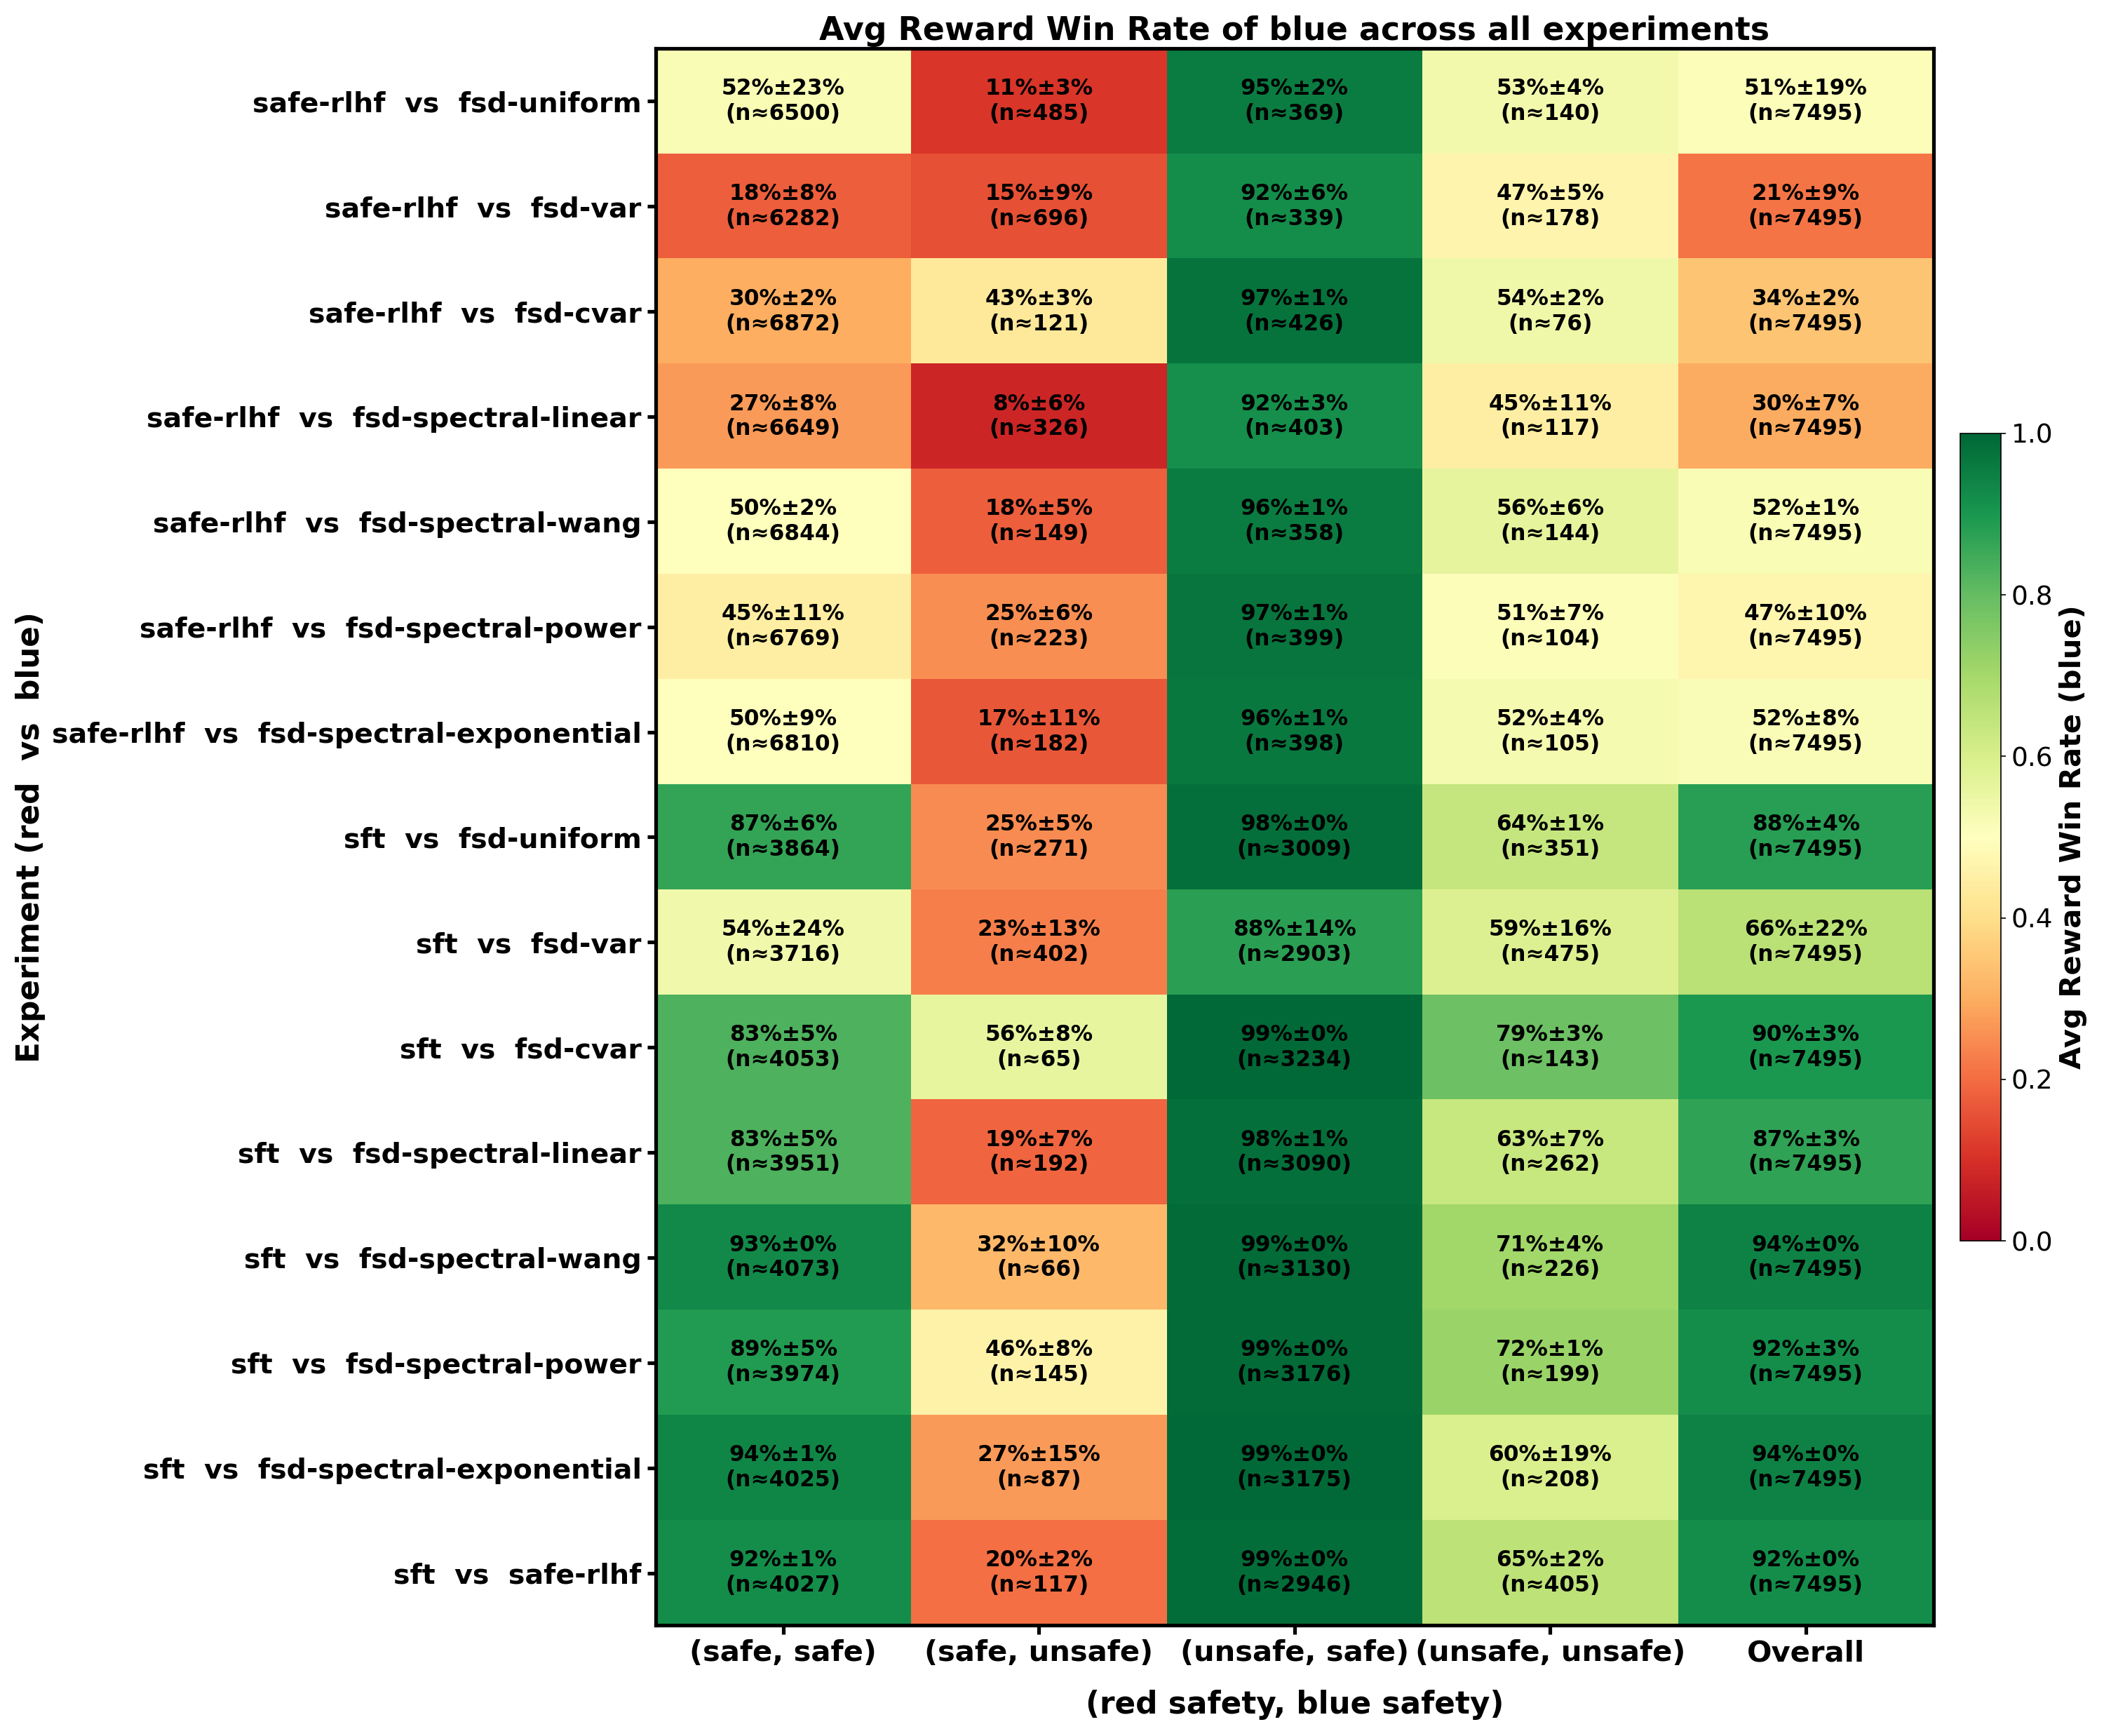
\includegraphics[width=0.9\textwidth]{./figs/summary_heatmap_averaged.png}
  \caption{
     Average reward win rates between competing models, across 3 seeds.
  }
  \label{fig:reward-winrates-test}
\end{figure}

\subsection{Out-of-Distribution Harmlessness: HarmBench Evaluation}

To assess generalization beyond the training distribution, we evaluate
all models on HarmBench \citep{mazeika2024harmbenchstandardizedevaluationframework}, an out-of-distribution
red-teaming benchmark comprising adversarially constructed harmful prompts
across diverse risk categories. Critically, neither the reward model, cost
model, nor any model checkpoint was trained or selected using HarmBench
data, making this a clean held-out evaluation.

We use GPT-4o-mini \citep{openai2024gpt4omini} as an independent pairwise harmlessness judge,
following standard LLM-as-a-judge \citep{zheng2023judgingllmasajudgemtbenchchatbot} evaluation protocol \cite{}. For each
prompt, the judge compares responses from two models and determines which
is less harmful. We provide the GPT evaluation results in \Cref{tab:harmbench-gpt-eval}

All RAD variants substantially outperform the SFT baseline, confirming that our constrained RL training, with the SFT policy as the reference, improves harmlessness and generalizes to unseen prompts.  Against Safe-RLHF, spectral variants -- Spectral-Power, Spectral-Exponential, Spectral-Linear, CVaR, and VaR -- achieve favorable win-loss ratios, suggesting that upweighting the tail of the cost distribution confers greater robustness to distributional shift. 

% \paragraph{Comparison against SFT.} All FSD variants substantially
% outperform the SFT baseline, with win rates ranging from 65.0\% to
% 82.4\% and loss rates below 31\%. This confirms that constrained RL
% training meaningfully improves harmlessness over supervised fine-tuning
% alone, and that this improvement generalizes to prompts unseen during
% training.

% \paragraph{Comparison against Safe RLHF.} Results are more nuanced
% when comparing against Safe RLHF. Some FSD variants — namely
% fsd-spectral-wang, fsd-spectral-exponential, fsd-spectral-power, fsd-spectral-linear, and fsd-cvar —
% achieve favorable win-loss ratios, indicating improved harmlessness
% generalization on OOD prompts. This suggests that spectral risk measures, which weight the
% tail of the cost distribution more heavily, confer greater robustness
% to distributional shift — consistent with our theoretical motivation for
% FSD-based constraints. Var should be in this list, but we obsderved that VaR suffers from unstable optimization, due to the dirac mass weighting

\begin{table}[t]
  \centering
  {\footnotesize
    \begin{tabular}{lcc}
      \toprule
      Model Name & SFT & Safe RLHF \\
      \midrule
      fsd-uniform & \underline{\textbf{67.1\%}}{\scriptsize$\pm$2.1} / 7.8\%{\scriptsize$\pm$4.2} / 25.1\%{\scriptsize$\pm$6.3} & 38.0\%{\scriptsize$\pm$6.9} / 22.2\%{\scriptsize$\pm$15.0} / \underline{\textbf{39.8\%}}{\scriptsize$\pm$8.4} \\
      fsd-var & \underline{\textbf{76.6\%}}{\scriptsize$\pm$3.7} / 10.6\%{\scriptsize$\pm$2.7} / 12.7\%{\scriptsize$\pm$2.3} & \underline{\textbf{39.6\%}}{\scriptsize$\pm$10.6} / 28.6\%{\scriptsize$\pm$16.8} / 31.8\%{\scriptsize$\pm$9.7} \\
      fsd-cvar & \underline{\textbf{72.9\%}}{\scriptsize$\pm$2.4} / 15.7\%{\scriptsize$\pm$1.3} / 11.4\%{\scriptsize$\pm$2.4} & \underline{\textbf{28.6\%}}{\scriptsize$\pm$7.8} / 46.5\%{\scriptsize$\pm$2.1} / 24.9\%{\scriptsize$\pm$6.6} \\
      fsd-spectral-linear & \underline{\textbf{75.3\%}}{\scriptsize$\pm$6.3} / 12.3\%{\scriptsize$\pm$2.0} / 12.4\%{\scriptsize$\pm$5.1} & \underline{\textbf{34.2\%}}{\scriptsize$\pm$2.8} / 37.0\%{\scriptsize$\pm$12.8} / 28.9\%{\scriptsize$\pm$13.4} \\
      fsd-spectral-wang & \underline{\textbf{67.3\%}}{\scriptsize$\pm$7.9} / 13.4\%{\scriptsize$\pm$0.6} / 19.3\%{\scriptsize$\pm$7.9} & 24.7\%{\scriptsize$\pm$1.7} / 49.7\%{\scriptsize$\pm$7.4} / \underline{\textbf{25.5\%}}{\scriptsize$\pm$8.1} \\
      fsd-spectral-exponential & \underline{\textbf{74.7\%}}{\scriptsize$\pm$1.6} / 12.6\%{\scriptsize$\pm$1.2} / 12.7\%{\scriptsize$\pm$1.6} & \underline{\textbf{28.0\%}}{\scriptsize$\pm$6.1} / 52.2\%{\scriptsize$\pm$7.0} / 19.9\%{\scriptsize$\pm$2.2} \\
      fsd-spectral-power & \underline{\textbf{71.0\%}}{\scriptsize$\pm$2.7} / 14.8\%{\scriptsize$\pm$2.1} / 14.1\%{\scriptsize$\pm$4.1} & \underline{\textbf{30.4\%}}{\scriptsize$\pm$2.0} / 48.9\%{\scriptsize$\pm$1.1} / 20.7\%{\scriptsize$\pm$2.7} \\
      \midrule
      Safe RLHF & \underline{\textbf{68.1\%}}{\scriptsize$\pm$2.6} / 20.4\%{\scriptsize$\pm$1.1} / 11.5\%{\scriptsize$\pm$2.5} & - \\
      \bottomrule
    \end{tabular}
  }
  \caption{
    Pairwise harmlessness evaluation on HarmBench using GPT-4o-mini as an independent judge. Each cell reports Win / Tie / Lose rates of the row model against the column model (mean $\pm$ std over 3 seeds). The dominant outcome -- win rate if the row model wins, loss rate if it loses -- is bold underlined. All FSD variants substantially outperform the SFT baseline. Against Safe RLHF, variants that upweight the tail (Eg: Exponential, Power, Linear, CVaR, and Var) achieve favorable win-loss ratios, demonstrating improved harmlessness generalization to out-of-distribution prompts.
  }
  \label{tab:harmbench-gpt-eval}
\end{table}


% \begin{table}[t]
%   \centering
%   {\footnotesize
%     \begin{tabular}{lcc}
%       \toprule
%       Model Name & SFT & Safe RLHF \\
%       \midrule
%       fsd-uniform & \underline{\textbf{67.1\%}}{\scriptsize$\pm$2.1} / 7.8{\scriptsize$\pm$4.2}\% / 25.1{\scriptsize$\pm$6.3}\% & 38.0{\scriptsize$\pm$6.9}\% / 22.2{\scriptsize$\pm$15.0}\% / \underline{\textbf{39.8\%}}{\scriptsize$\pm$8.4} \\
%       fsd-var & \underline{\textbf{76.6\%}}{\scriptsize$\pm$3.7} / 10.6{\scriptsize$\pm$2.7}\% / 12.7{\scriptsize$\pm$2.3}\% & \underline{\textbf{39.6\%}}{\scriptsize$\pm$10.6} / 28.6{\scriptsize$\pm$16.8}\% / 31.8{\scriptsize$\pm$9.7}\% \\
%       fsd-cvar & \underline{\textbf{72.9\%}}{\scriptsize$\pm$2.4} / 15.7{\scriptsize$\pm$1.3}\% / 11.4{\scriptsize$\pm$2.4}\% & \underline{\textbf{28.6\%}}{\scriptsize$\pm$7.8} / 46.5{\scriptsize$\pm$2.1}\% / 24.9{\scriptsize$\pm$6.6}\% \\
%       fsd-spectral-linear & \underline{\textbf{75.3\%}}{\scriptsize$\pm$6.3} / 12.3{\scriptsize$\pm$2.0}\% / 12.4{\scriptsize$\pm$5.1}\% & \underline{\textbf{34.2\%}}{\scriptsize$\pm$2.8} / 37.0{\scriptsize$\pm$12.8}\% / 28.9{\scriptsize$\pm$13.4}\% \\
%       fsd-spectral-wang & \underline{\textbf{67.3\%}}{\scriptsize$\pm$7.9} / 13.4{\scriptsize$\pm$0.6}\% / 19.3{\scriptsize$\pm$7.9}\% & 24.7{\scriptsize$\pm$1.7}\% / 49.7{\scriptsize$\pm$7.4}\% / \underline{\textbf{25.5\%}}{\scriptsize$\pm$8.1} \\
%       fsd-spectral-exponential & \underline{\textbf{74.7\%}}{\scriptsize$\pm$1.6} / 12.6{\scriptsize$\pm$1.2}\% / 12.7{\scriptsize$\pm$1.6}\% & \underline{\textbf{28.0\%}}{\scriptsize$\pm$6.1} / 52.2{\scriptsize$\pm$7.0}\% / 19.9{\scriptsize$\pm$2.2}\% \\
%       fsd-spectral-power & \underline{\textbf{71.0\%}}{\scriptsize$\pm$2.7} / 14.8{\scriptsize$\pm$2.1}\% / 14.1{\scriptsize$\pm$4.1}\% & \underline{\textbf{30.4\%}}{\scriptsize$\pm$2.0} / 48.9{\scriptsize$\pm$1.1}\% / 20.7{\scriptsize$\pm$2.7}\% \\
%       Safe RLHF & \underline{\textbf{68.1\%}}{\scriptsize$\pm$2.6} / 20.4{\scriptsize$\pm$1.1}\% / 11.5{\scriptsize$\pm$2.5}\% & - \\
%       \bottomrule
%     \end{tabular}
%   }
%   \caption{
%     Pairwise harmlessness evaluation on HarmBench using GPT-4o-mini as an independent judge. Each cell reports Win / Tie / Lose rates of the row model against the column model (mean $\pm$ std over 3 seeds). The dominant outcome -- win rate if the row model wins, loss rate if it loses -- is bold underlined. All FSD variants substantially outperform the SFT baseline. Against Safe RLHF, variants that upweight the tail (Eg: Exponential, Power, Linear, CVaR, and VaR) achieve favorable win-loss ratios, demonstrating improved harmlessness generalization to out-of-distribution prompts.
%   }
%   \label{tab:harmbench-gpt-eval}
% \end{table}


% \begin{table}[t]
%   \centering
%   {\footnotesize
%     \begin{tabular}{lcc}
%       \toprule
%       Model Name & SFT & Safe RLHF \\
%       \midrule
%       fsd-uniform & \underline{\textbf{65.0\%}} / 4.3\% / 30.7\% & 44.5\% / 4.9\% / \underline{\textbf{50.6\%}} \\
%       fsd-var & \underline{\textbf{71.6\%}} / 14.2\% / 14.2\% & 24.7\% / 48.2\% / \underline{\textbf{27.1\%}} \\
%       fsd-cvar & \underline{\textbf{76.0\%}} / 14.6\% / 9.4\% & \underline{\textbf{39.7\%}} / 44.7\% / 15.6\% \\
%       fsd-spectral-linear & \underline{\textbf{82.4\%}} / 11.9\% / 5.7\% & \underline{\textbf{37.9\%}} / 45.1 \% / 17.0 \% \\
%       fsd-spectral-wang & \underline{\textbf{69.2\%}} / 12.6 \% / 18.2 \% & \underline{\textbf{27.1\%}} / 54.1\% / 18.8\% \\
%       fsd-spectral-exponential & \underline{\textbf{72.8\%}} / 12.1 \% / 15.0\% & \underline{\textbf{22.6\%}} / 60.4\% / 17.0\% \\
%       fsd-spectral-power & \underline{\textbf{69.6 \%}} / 11.8 \% / 18.6\% & \underline{\textbf{30.8\%}} / 47.7\% / 21.5\% \\
%       Safe RLHF & \underline{\textbf{67.4\%}} / 22.0 \% / 10.6 \% & - \\
%       \bottomrule
%     \end{tabular}
%   }
%   \caption{
%     Pairwise harmlessness evaluation on HarmBench using GPT-4o-mini as an independent judge. Each cell reports Win / Tie / Lose rates of the row model against the column model. The dominant outcome -- win rate if the row model wins, loss rate if it loses -- is bold underlined. All FSD variants substantially outperform the SFT baseline. Against Safe RLHF, variants that upweight the tail (Wang, Exponential, Power, Linear, and CVaR) achieve favorable win-loss ratios, demonstrating improved harmlessness generalization to out-of-distribution prompts.
%   }
%   \label{tab:harmbench-gpt-eval}
% \end{table}
